\documentclass[aspectratio=169,11pt]{beamer}

\usetheme{default}
\usepackage[T1]{fontenc}
\usepackage{lmodern}
\usepackage{microtype}
\usepackage{amsmath,amssymb}
\usepackage{booktabs}
\usepackage{array}
\usepackage{graphicx}
\usepackage{tikz}
\usetikzlibrary{arrows.meta,positioning}

\definecolor{Primary}{HTML}{2C5F52}
\definecolor{Secondary}{HTML}{B8860B}
\definecolor{TitleBg}{HTML}{1F4037}
\definecolor{ProblemBg}{HTML}{FAF7F0}

\setbeamercolor{normal text}{fg=black!88!white,bg=white}
\setbeamercolor{structure}{fg=Primary}
\setbeamercolor{frametitle}{fg=Primary,bg=white}
\setbeamercolor{footline}{fg=Primary!75!white}
\setbeamerfont{frametitle}{series=\bfseries,size=\Large}
\setbeamersize{text margin left=7mm,text margin right=7mm}

\setbeamertemplate{navigation symbols}{}
\setbeamertemplate{itemize item}{\textcolor{Secondary}{\rule[0.35ex]{0.55ex}{0.55ex}}}
\setbeamertemplate{itemize subitem}{\textcolor{Secondary!70}{--}}
\setbeamertemplate{frametitle}{%
  \vspace*{2.4mm}%
  {\usebeamerfont{frametitle}\usebeamercolor[fg]{frametitle}\insertframetitle\par}%
  \vspace*{0.3mm}{\color{Secondary}\rule{18mm}{1pt}\par}\vspace*{0.6mm}%
}
\setbeamertemplate{footline}{%
  \hbox to\paperwidth{\hspace{7mm}%
    \scriptsize\color{Primary!70!white}Chrysafis / Zhou \textbullet\ CS 566%
    \hfill\scriptsize\insertframenumber\hspace{7mm}}%
  \vspace{1.6mm}%
}

\newcommand{\captext}[1]{{\fontsize{7.5}{9}\selectfont\itshape\color{black!60}#1\par}}
\newcommand{\head}[1]{{\bfseries\color{Primary}#1}}

\begin{document}

% ---------- 1. Title ----------
{
\setbeamercolor{background canvas}{bg=TitleBg}
\begin{frame}[plain]
\vspace{16mm}
{\color{Secondary}\rule{20mm}{1.2pt}\par}\vspace{4mm}
{\color{white}\LARGE\bfseries Monocular Depth Estimation:\par}\vspace{1mm}
{\color{white}\LARGE\bfseries Benchmarking and a Defocus-Informed Refinement\par}
\vspace{7mm}
{\color{white!85!TitleBg}\large Dimitri Chrysafis \quad Vincent Zhou\par}
\vspace{3mm}
{\color{white!60!TitleBg}\normalsize COMPSCI 566 \textbullet\ Fall 2026 \textbullet\ December 1\par}
\end{frame}
}

% ---------- 2. Problem ----------
\begin{frame}{One image cannot give meters}
\begin{columns}[T]
\column{0.55\linewidth}
\begin{itemize}\setlength{\itemsep}{5pt}
\item A small nearby object and a large far one project identically: learned depth is defined only up to scale and shift.
\item Result: per-image alignment is required before a relative model can report meters.
\item Defocus is different: blur is set by thin-lens geometry, so a focal stack carries an absolute scale cue.
\end{itemize}
\column{0.42\linewidth}
\centering
\vspace{1mm}
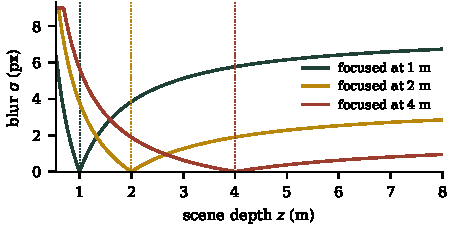
\includegraphics[width=\linewidth]{figs/blur_curve.pdf}\\[2pt]
\captext{Blur $\sigma$ vs.\ scene depth for three focus settings. The curve is anchored in meters, not relative units.}
\end{columns}
\end{frame}

% ---------- 3. Pipeline ----------
\begin{frame}{Three components, one depth map}
\begin{center}
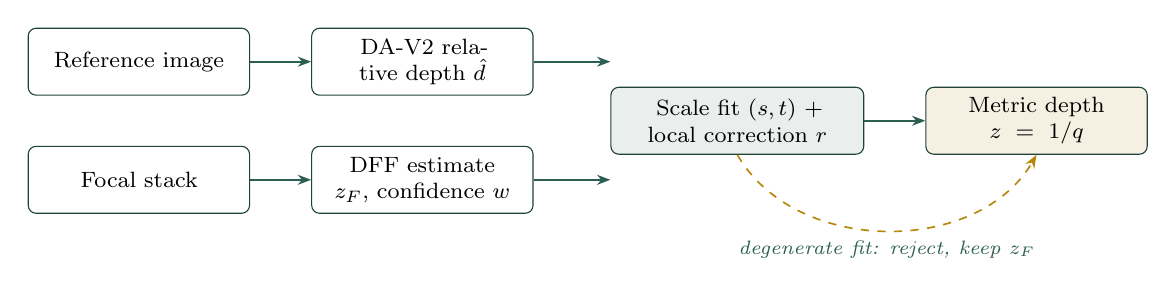
\begin{tikzpicture}[font=\footnotesize,
  box/.style={draw=Primary!70!black,fill=white,rounded corners=1mm,minimum height=8.5mm,text width=26mm,align=center,inner sep=3pt},
  arr/.style={-{Stealth[length=1.7mm]},draw=Primary,semithick}]
\node[box] (rgb)  at (0,0)    {Reference image};
\node[box] (net)  at (3.6,0)  {DA-V2 relative depth $\hat d$};
\node[box] (stk)  at (0,-1.5) {Focal stack};
\node[box] (dff)  at (3.6,-1.5){DFF estimate $z_F$, confidence $w$};
\node[box,fill=Primary!10,text width=30mm] (fit) at (7.6,-0.75) {Scale fit $(s,t)$ + local correction $r$};
\node[box,fill=Secondary!12] (out) at (11.4,-0.75) {Metric depth $z=1/q$};
\draw[arr] (rgb)--(net);
\draw[arr] (stk)--(dff);
\draw[arr] (net.east)--(fit.west|-net.east);
\draw[arr] (dff.east)--(fit.west|-dff.east);
\draw[arr] (fit)--(out);
\draw[arr,draw=Secondary,dashed] (fit.south) to[out=-60,in=-120] node[below,pos=0.5,font=\scriptsize\itshape,text=Primary]{degenerate fit: reject, keep $z_F$} (out.south);
\end{tikzpicture}
\end{center}
\vspace{1mm}
\begin{itemize}\setlength{\itemsep}{3pt}
\item \head{Learned branch:} Depth Anything V2 (ViT-S/B/L + metric indoor checkpoint), evaluated on 654 NYU-Depth v2 test images.
\item \head{Classical branch:} depth from focus on rendered stacks (6 scenes, tune/eval split) and DDFF 12-Scene (120 real stacks).
\item \head{Ours:} focus-informed scale fitting and regularized refinement, with rejection and a focus fallback.
\end{itemize}
\end{frame}

% ---------- 4. NYU baseline ----------
\begin{frame}{Learned baseline: alignment is the whole game}
\begin{columns}[T]
\column{0.56\linewidth}
\vspace{1mm}
{\scriptsize\setlength{\tabcolsep}{4pt}
\begin{tabular}{llccc}
\toprule
Checkpoint & Alignment & AbsRel & RMSE (m) & $\delta_1$ \\
\midrule
ViT-S & median scale & 0.494 & 2.349 & 0.393 \\
ViT-S & least squares & 0.062 & 0.297 & 0.956 \\
ViT-S & robust IRLS & 0.058 & 0.292 & 0.958 \\
ViT-B & least squares & 0.057 & 0.283 & 0.959 \\
ViT-L & least squares & \textbf{0.055} & \textbf{0.277} & \textbf{0.961} \\
Metric-Indoor-S & none (raw) & 0.218 & 0.650 & 0.670 \\
Metric-Indoor-S & least squares & 0.077 & 0.353 & 0.936 \\
\bottomrule
\end{tabular}\par}
\vspace{2pt}
\captext{NYU-Depth v2 test split, 654 images, Eigen crop.}
\column{0.42\linewidth}
\centering
\vspace{1mm}
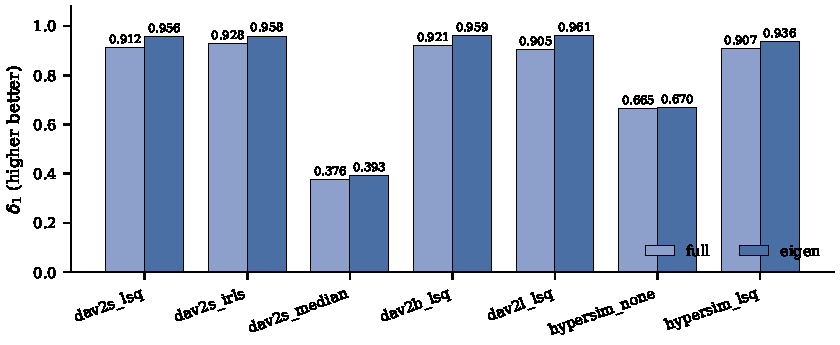
\includegraphics[width=\linewidth]{figs/nyu_models.pdf}\\
\captext{$\delta_1$ by checkpoint, full vs.\ Eigen crop.}
\end{columns}
\vspace{2mm}
\begin{itemize}\setlength{\itemsep}{2.5pt}
\item Median scale collapses (0.494): a scalar cannot fix inverse-depth offset. Affine $q=s\hat d+t$ is the minimum.
\item The metric checkpoint has a scale prior but is biased on NYU: 0.218 raw vs.\ 0.077 aligned.
\item S $\to$ L buys $\approx$0.005 $\delta_1$ at ${\sim}4\times$ runtime: ViT-S is our refinement backbone.
\end{itemize}
\end{frame}

% ---------- 5. DFF ----------
\begin{frame}{Depth from focus on synthetic stacks}
\begin{center}
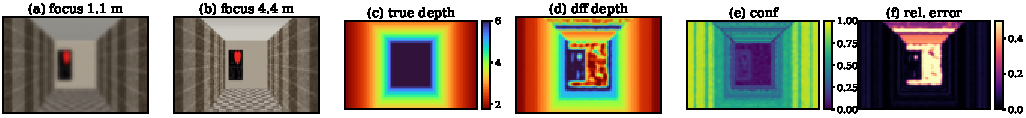
\includegraphics[width=\linewidth]{figs/synth_dff_corridor.pdf}\\[1pt]
\captext{Corridor: two focus slices, ground-truth depth, DFF estimate, confidence, relative error.}
\end{center}
\vspace{0.5mm}
\begin{itemize}\setlength{\itemsep}{2.5pt}
\item Modified Laplacian focus measure per frame; parabolic fit around the peak gives sub-frame $z_F$.
\item Confidence $w\in[0,1]$ marks flat or ambiguous focus curves; $\bar w\approx0.06$--0.26 textureless vs.\ 0.26--0.66 textured.
\item All-focus guided smoothing in inverse depth recovers flat regions (textureless AbsRel $0.77\to0.61$ held out).
\item Accurate where texture exists; degrades on flat surfaces and at occlusion boundaries (defocus veiling).
\end{itemize}
\end{frame}

% ---------- 6. Scale fit + refinement ----------
\begin{frame}{Contribution: defocus-informed scale fitting}
\vspace{1mm}
Affine fit on inverse depth plus a local correction $r$:
\[
q(\mathbf{x})=s\,\hat d(\mathbf{x})+t+r(\mathbf{x}),\qquad z(\mathbf{x})=q(\mathbf{x})^{-1}
\]
\[
\min_{s,t,r}\;\sum_{\mathbf{x}} w(\mathbf{x})\,\rho\!\left(q(\mathbf{x})-z_F(\mathbf{x})^{-1}\right)
+\lambda\sum_{\mathbf{x}}\|\nabla r(\mathbf{x})\|^2
+\mu\sum_{\mathbf{x}} r(\mathbf{x})^2,
\qquad q\geq\epsilon>0
\]
\vspace{1mm}
\begin{itemize}\setlength{\itemsep}{3pt}
\item Huber loss $\rho$, confidence-weighted: only reliable focus pixels pull the fit.
\item Affine $(s,t)$ first with $r=0$, then local corrections; $\lambda,\mu$ suppress large or abrupt edits where $w$ is weak.
\item \head{Rejection:} anticorrelated predictions make the fit degenerate ($s\le0$); the output is marked uncalibrated and falls back to $z_F$ instead of emitting bad metric depth.
\end{itemize}
\end{frame}

% ---------- 7. Synthetic results ----------
\begin{frame}{Held-out synthetic scenes: combined beats both parts}
\begin{columns}[T]
\column{0.54\linewidth}
\vspace{1mm}
{\scriptsize\setlength{\tabcolsep}{4pt}
\begin{tabular}{lccc}
\toprule
Method & AbsRel & RMSE (m) & $\delta_1$ \\
\midrule
DFF raw & 0.233 & 1.552 & 0.732 \\
DFF + all-focus smoothing & 0.221 & 1.510 & 0.702 \\
DA-V2 aligned (oracle) & 0.271 & 1.524 & 0.548 \\
DA-V2 + scale fit & 0.308 & 1.614 & 0.459 \\
Refined (ours) & 0.259 & 1.483 & 0.575 \\
Combined (ours) & \textbf{0.206} & \textbf{1.284} & 0.704 \\
\bottomrule
\end{tabular}\par}
\vspace{2pt}
\captext{Mean over 4 held-out scenes (corridor, objects, slanted, shelves); weights tuned on gallery + stairs only. Metric depth scored without alignment.}
\column{0.44\linewidth}
\centering
\vspace{1mm}
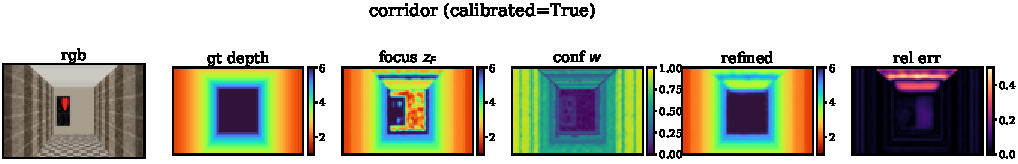
\includegraphics[width=\linewidth]{figs/refine_corridor.pdf}\\[1pt]
\captext{Corridor: refined depth (calibrated).}
\begin{itemize}\setlength{\itemsep}{2pt}\footnotesize
\item Combined $=$ refined when calibrated, focus estimate when rejected.
\item Per scene it matches the better component; on the mean it beats both.
\end{itemize}
\end{columns}
\end{frame}

% ---------- 8. Rejection / failure ----------
\begin{frame}{When the fit fails, say so}
\begin{center}
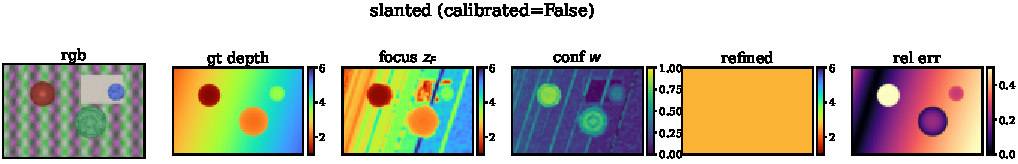
\includegraphics[width=\linewidth]{figs/refine_slanted.pdf}\\[1pt]
\captext{Slanted (calibrated = False): DA-V2 output anticorrelates with the focus estimate, $s\le0$, so the refinement is rejected and the combined output returns $z_F$.}
\end{center}
\vspace{1.5mm}
\begin{itemize}\setlength{\itemsep}{3pt}
\item Scale fit alone on this scene: AbsRel 0.297 vs.\ focus estimate 0.087. The fallback is what makes the combined row win.
\item Also exposed: defocus veiling lifts $w$ near depth edges, and 2--3-frame stacks collapse the focus estimate entirely (AbsRel $>$10).
\end{itemize}
\end{frame}

% ---------- 9. DDFF ----------
\begin{frame}{Real stacks: DDFF 12-Scene, qualitative only}
\begin{center}
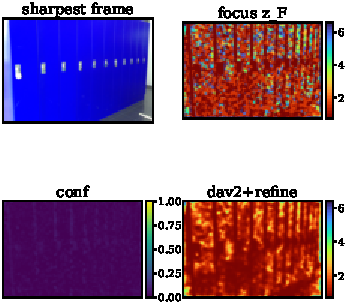
\includegraphics[height=29mm]{figs/ddff_refine_test_000.pdf}\hfill
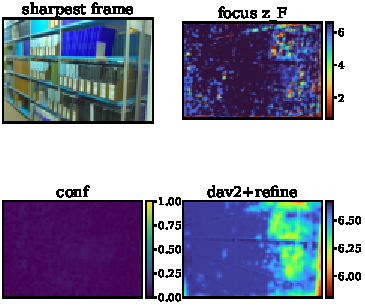
\includegraphics[height=29mm]{figs/ddff_refine_test_044.pdf}\hfill
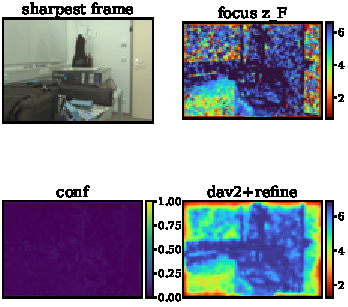
\includegraphics[height=29mm]{figs/ddff_refine_test_072.pdf}
\end{center}
\captext{Sharpest frame, focus estimate, confidence, DA-V2 + refinement on three DDFF test stacks.}
\vspace{0.4mm}
\begin{itemize}\setlength{\itemsep}{2pt}
\item 120 Lytro stacks, no public ground truth (withheld for the benchmark server): qualitative evaluation only.
\item Focus distances are not recorded; we rebuilt them from the paper's refocus geometry and verified ordering per stack.
\item Real-stack confidence is low ($\bar w\approx0.02$--0.05); per-scene confidence normalization gets calibration accepted on most stacks.
\end{itemize}
\end{frame}

% ---------- 10. Takeaway ----------
\begin{frame}{Takeaway, limitations, next}
\begin{itemize}\setlength{\itemsep}{5pt}
\item \head{Benchmark:} relative DA-V2 is excellent after affine alignment (NYU $\delta_1$ 0.961) but the metric checkpoint (0.218) and median scaling (0.494) are not safe defaults.
\item \head{Contribution:} focus gives absolute scale where texture exists; confidence-weighted fitting plus rejection turns it into a usable metric prior. Held-out AbsRel 0.206 beats DFF (0.233) and aligned DA-V2 (0.271).
\item \head{Limitations:} texture dependence, veiling at occlusion edges, no DDFF ground truth, synthetic gap to real cameras.
\item \head{Next:} more DDFF stacks, phone-captured focal stacks, per-checkpoint runtimes on the webpage.
\end{itemize}
\vspace{4mm}
\centering\footnotesize\color{Primary!80!white}
github.com/DimitriChrysafis/cs566-project \textbullet\ questions in the live Q\&A
\end{frame}

\end{document}
